\documentclass[12pt]{extarticle}
\usepackage[utf8]{inputenc}
\usepackage[T1]{fontenc}
\usepackage[english]{babel}
\usepackage{natbib}
\usepackage{gensymb}
\usepackage{graphicx}
\graphicspath{ {./images/} }
\bibliographystyle{apa}

%%%%%%%%%%%%%%%%%%%%%%%%%%%%%%%%%
%Delimitation of the project and working title for the thesis.
%Theoretical hypothesis and/or research question.
%Aim, value and expected impact of the project.
%Scope and timeplan of the project.
%References and materials, the student‘s status of relevant knowledge
%Research method, data collection and analysis, scope and timeframe.
%uggested table of contents for the thesis.%

\title{Parental Effects on Development and Behavior in Threespine Stickleback \textit{Gasterosteus aculeatus} of Lake M\'yvatn, Iceland}
\author{Spencer Edwards, Roll No.}
\date{April 2021}

\begin{document}

\maketitle

\section*{Research Question}
Major questions I want to address:
\begin{itemize}
 \item To what extent is phenotypic divergence of lake M\'yvatn stickleback from cold and warm habitats
shaped by maternal and paternal (parental) effects?
 \item Specifically, how much variation in stickleback phenotypes  of morphology (For example:  shape, feeding structures), phenology (growth rate, size,  and behavior (For example: feeding behavior, anti predator behavior, shyness/boldness, shoaling) are driven by direct genetic effects, parental effects, and environmental effects experienced during development? How does this translate to adult sub-populations?
 \item How do parental effects influence adaptive divergence in M\'yvatn stickleback? To what extent does environmental variation (for instance, water temperature) play in this divergence?
\end{itemize}

\section*{Relevant Background}
\paragraph{Introduction}
The central question of evolutionary biology involves understanding the causes and consequences of phenotypic variation, and how this results in new species. Over the past several decades, much thought has been put into the relationship between development and evolution and their impact on said variation.
The traits gained by an organism from its parents during development and early life history are key to its success as an individual. It is not surprising then, that parental effects, both maternal and paternal, have a major impact on organisms and their evolution \citep{charmantier_garant_kruuk_2014, Danchin2011, Badyaev2009}. When considering the sources of phenotypic variation, parental effects on phenotype, and particularly their impacts on eco-evolutionary dynamics, stand out as topics that have gained relatively less attention amongst the evo-devo community. Parental effects, defined as a change in an offspring's phenotype due to the phenotype and/or environment of one or more of its parents, were for a long time considered a nuisance, a deviation from pure heritable traits. Now however we have seen a resurgence of interest in these effects \citep{charmantier_garant_kruuk_2014}.
Parental effects are of particular interest to evolutionary ecologists because they have the ability to both promote rapid phenotypic diversification and integration, as well as prevent it through matching developmental gene expression and timing \citep{Badyaev2009}. When quantifying parental effects, we first need to establish if parental effects are expressed, and if so, where in the life-history of the organism they are expressed. From there we can use more advanced genetic techniques to parse out the exact origin of the effects we are interested in. While much research has been done concerning the impact of parental effects on development \citep{Tigreros2021} and behavior of invertebrates (particularly beetles), comparatively less is known about parental effects on vertebrates. Work on teleosts has revealed strong links between parental effects on the co-evolution of behavior and cellular function \citep{Yoshizawa2012}. The connection between parental affects influencing behavior and gene expression has serious implications for evolutionary ecology, because rapid environmental could act as a mechanism for rapid evolution via parental programming of offspring phenotypes, effectively providing their offspring with a ``jump start'' of sorts \citep{Danchin2011, Donelson2018}. 
\paragraph{Quantitative Genetics}
One of the most powerful ways of analyzing sources of phenotypic variance is quantitative genetics. Quantitative genetics is, as the name suggests, a way of quantifying phenotypic traits from genetic and non-genetic sources \citep{Wilson2010}.
From the standpoint of quantitative genetics, the phenotype (\textit{P}) is equal to the influence of genes (\textit{G}) and environment (\textit{E}) such that $$P = G + E $$

However, genetic effects from parents can be further broken down into inheritance from genes directly ($I_G$) and inheritance from the parental environment ($I_E$) such that $$P = (I_G + I_E) + G \times E$$

Quantitative genetics uses the relationships between relatives to analyze sources of phenotypic variation, in particular the phenotypic variation caused by complex traits.
The benefit of using a quantitative genetics model is that we can make predictions about where traits come from and test them using a Generalized Linear Mixed Model (GLMM) \citep{Wilson2010, Bolker2009, VanDooren2016}. GLMMs allow us to estimate how much of the phenotype is derived from genetics by breaking down the variance of the phenotype into multiple sources. By portioning the phenotypic variance into genetic and environmental effects (Sometimes referred to as Additive and Residual, respectively), we can extend our analysis to multiple co-varying traits and analyze where multiple traits which are responsible for differences in life-history strategies come from. From there, we can make predictions about how phenotypes will evolve. This is important for management decisions in an era of rapid global climate change \citep{VanDooren2016}.

\paragraph{The Lake M\'yvatn Ecosystem}
Here in Iceland, work on various populations of \textit{Gasterosteus aculeatus} has focused on phenotypic diversity, including phenotypic plasticity \citep{Kristjansson2002, Millet2013}. Icelandic stickleback show high levels of genetic variation, implying a single colonization and spread by marine stickleback \citep{Olafsdottir2007}. Particularly in neo-volcanic lakes, resource polymorphism has driven the evolution of sympatric ecotypes \citep{Olafsdottir2007, Kristjansson2002} that show a high degree of morphological and behavioral divergence occurring over a relatively short amount of time (100 years) \citep{Lucek2014}. Lake M\'yvatn stickleback in particular provide an excellent study system for uncovering the sources of phenotypic divergence, due to its complex habitats. There is a large difference between various basins of the lake, owing to variation in sediment composition, temperature, prey, and predator populations. Prey populations, including the chironomid \textit{Tanytarsus gracilentus}, can fluctuate up to seven orders of magnitude over time \citep{Bartrons2018}.  Water temperatures between the basins are fed by hot and cold springs, leading to stark differences in temperature \citep{Einarsson2004}. Unlike other arctic and subarctic lakes, M\'yvatn is eutrophic, and its community is driven by consumer-resource as well as predator-prey interactions \citep{Bartrons2018}, resulting in uneven distributions of primary producers \citep{Einarsson2004}. Furthermore, predator populations including \textit{Salvelinus alpinus} and \textit{Salmo trutta} are not evenly dispersed throughout the lake. These factors, combined with the lack of physical dispersal barriers, indicates a high potential for divergent selection while also retaining high amounts of gene flow. However, the extent to which parental effects shape the morphology and behavior of lake M\'yvatn stickleback has yet to be investigated fully. Gaining a holistic understanding of the causes to consequences of phenotypic divergence and intraspecific variation is a necessary precursor to assessing how a system will respond in the future.
\paragraph{Parental Effects}
Previous work on different stickleback populations have discovered a range of parental effects, both maternal and paternal. \citet{Bell2018} investigated the heritability of parental behavior (Specifically, fanning of eggs) by male stickleback and found strong heritability of the trait. Furthermore, they concluded that a strong amount of genetic variation could lead the evolvability of the fanning trait. Offspring of male stickleback that experience predation risk have shown to grow smaller and spend less time in the open \citep{Bell2016, Stein2014} Female stickleback have also been shown to pass on phenotypic information to their eggs. An RNAseq study analyzing female stickleback found that eggs from mothers exposed to predators had faster development times, as well as major epigenetic changes and alterations to non-coding genes during development \citep{Mommer2014, Bell2016}. Environmental components can play a role in shaping parental effects as well. Parental effects can be more or less pronounced depending on resource availability and temperatures experienced by parents and offspring during development \citep{Rasanen2007} and should therefore be divergent in complex habitats like lake M\'yvatn. Parental effects often occur with parent-offspring conflicts, which occur when there is a discrepancy between life-history strategies that result in higher fitness for either parents or offspring \citep{Uller2008}. For example, maternal fitness of oviparous organisms will often increase with increasing numbers of eggs laid, however each egg then gets less nutrients allocated to it by its mother, reducing the individual offspring's fitness \citep{Uller2008, Rasanen2007}. Filial cannibalism may also play a role in increasing the survival of the remaining offspring in a density-dependent system and during times of low food availability \citep{Bartrons2018} \\
Parental effects of lake M\'yvatn stickleback and their impact of offspring fitness have been the subject of multiple master's theses, however there are still major gaps in our knowledge. In particular, we have little data on parental effects on offspring performance during their adult lives, and any environmental interactions (in particular, contrasting temperature regimes) have yet to be fully explored. For example, \citet{Senn} found that female investment differed between cold and warm morphs in egg number, egg size, clutch mass, and males had higher fanning activity in warm treatments. As a follow up, \citet{Diethelm} found no evidence of maternal effects on overall offspring survival as \citet{Senn} had. However, they weren't able to investigate the development and behavior of offspring, particularly in contrasting temperatures. They also noted that it would be interesting to test if offspring from cold water mothers, when raised in warm temperatures, experience enhanced abnormalities as a result of faster development. Taken together, these results show a gap in our knowledge regarding the nature of parental effects in M\'yvatn stickleback. What's more, neither of these works examined the relationship between parental effects and divergence in the context of a highly variable sympactric population.

\paragraph{The Role of Temperature Variation}
Temperature variation has a large impact on the development of ectotherms including fishes \citep{Massey2021}. Nonlinear temperature effects have been shown to lead to variation in canalization of phenotypic traits in stickleback \citep{Ramler2014}. Furthermore, some stickleback populations demonstrate environment-specific maternal effects in offspring growth, Particularly in early development \citep{Ramler2014, Shama2014b}.

\paragraph{Hypotheses}
The impact of parental effects on post-hatching development and behavior of stickleback has yet to be described. Moreover, whether M\'yvatn stickleback morphs differ in maternal investment has yet to be conclusively determined. 
If parental effects are present and result in adaptive divergence, then we should expect to see hybrids form an intermediate between the two phenotypes expressed. I predict that cold mothers will produce more offspring than warm mothers. Fish from warm mothers, when raised in cold temperatures, should experience stunted development (slower development time and smaller size), whereas fish from cool mothers, when raised in warm temperatures, should experience faster development and larger size and birth defects.
According to \citet{Senn} we should also see differences in surviving offspring between treatments, with higher numbers for cold mother offspring raised in cold water and vice versa. hybrids should be intermediate in growth rate and size.


%Danchin2011 discusses some evidence for non-genetic inheritence mechanisms and calls for a new extended synthesis %
%rasanen et al consider evidence that maternal effects are not entriely environmental but that the environment does play a cruicial role in determining the impact of these affects, and lays out evidence and examples on an ecological time scale



\section*{Methods}

\paragraph{Collection}
Fish will be collected from two stations at lake M\'yvatn: Grimsstaðir, a cool portion of the north basin, and Hot Shore, a warm portion. Fish will be caught using mesh nets and kept in tanks while being transported to Verið Research Station in Sauðárkrókur, Iceland. Adult fish will be kept in tanks at Verið until crosses are performed.

\paragraph{Crosses}
Female will will be checked every day for gravidity. When gravid fish are found, they will be crossed.
Crosses will be performed using a modified method based on Schluter. One male and One female fish are obtained and placed in small buckets with water the same temperature as the system (13 \degree C), along with 1 ml Ginsenburg solution for testes (two total) in 2 ml eppendrof tubes. Phenoxyethnol will be used to anesthetise fish. Males are anesthetized, weighed and recorded, and photographed (see Photography section). Gonads are dissected via the following method:
Fish are held and an incision is made along the cloaca with dissecting scissors. A cut is made upwards, towards the lateral line, and then along the lateral line towards the pectoral fine. Fine curved forceps are used to identify and remove testes. Once removed, they are placed in Ginsenburg solution.
Testes are crushed using forceps to release the sperm. The male's spine is sniped to ensure death. Once death has been ensured, a fin clip is taken and placed in a bag containing the fish ID for genetic analysis.
Females are weighed pre-stripping on a digital scale, recorded, and stripped into a dry petri dish using the following method:
Fish are held gently and the cloaca massaged to release the eggs into a small petri dish. After stripping, the female is weighed again, aanesthetized with Phenoxyethnol and killed by snipping the spinal chord. The egg mass is split placed in the Ginsenburg solution for fertilization.
 The eggs are allowed to rest for 10 minutes before being placed in a petri dish and covered with water. Eggs are allowed to rest again for 20 minutes, the water is removed and replaced with fresh water, then allowed to rest for 30 minutes (for a total of 1 hour), before being checked under a microscope for complete fertilization. When fertilization is confirmed, the egg mass will be split in half for the temperature treatments before being taken downstairs and placed in breeding tanks (see below)
 
\paragraph{Experimental Design}
I will utilize an independent line cross, $2 \times 2 \times 4$ factorial randomized block experiment to assess parental effects in Mývatn stickleback, with two populations, 2 temperature treatments (13 \degree C and 17 \degree C) and four cross types (CC, CH, HC, HH). Stickleback will be collected from Grímsstaðir and hot shore at lake M\'yvatn. Sticklebacks from both shores will then be crossed using standard methods laid out by Schluter. Each cross uses unique individuals only, with 8 crosses per cross type, for a total of 32 crosses. We chose independent line crosses due to space constraints, as well as maximizing the number of offspring created. independent line crossing has been used with stickleback previously to quantify morphological divergence \citep{Berner2011}. Factorial designs have been used previously to examine the effects of indirect fitness in parasite resistance, as well as transgenerational plasticity in response to temperature in marine stickleback (Barber et al. 2001; Ramler et al. 2014). Once incubated, eggs will be randomly assigned tank number. Single families will be placed in two separate tanks to test for influence of temperature on parental effects and development of offspring. A total of 80 tanks will be used to house the 40 families. Juvenile fish will be fed artemia until fully grown. Adult fish will be raised in 10L tanks in a common garden at 13 °C and fed a mixed diet of blood worms (twice a day Tues and Thurs) and pellets (once a day, Mon, Wed, Fri). Fish will be weighed/measured every 3 months until fully grown, when their behavior will be assessed. 


\paragraph{Statistics} One of the major problems when considering historical work on parental effects is disentangling genetic and environmental effects (Donelson et al. 2018). Using a Linear Mixed Model (LMM) approach to decompile the effects will 

\begin{figure}
\centering
 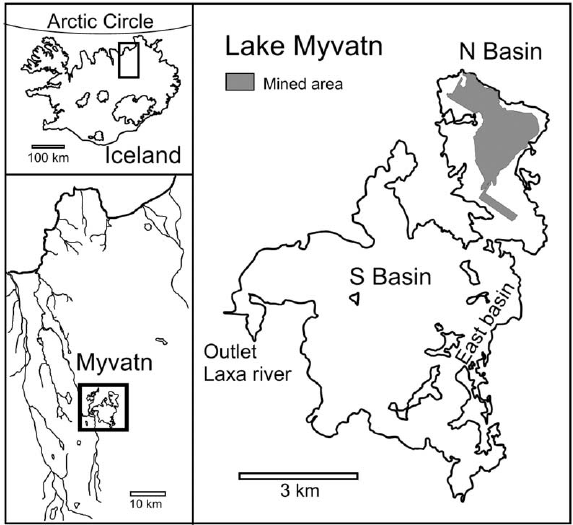
\includegraphics[width=0.7\textwidth]{lake}
 \caption{Map of lake M\'yvatn. Taken from \citet{Einarsson2004}}
  \label{fig:pedigree1}
\end{figure}

\section{Timeline}
Collection of breeding fish will begin on the 2nd of July and takes about 2 days. Fish will be collected and transported to Verið on the 3rd of July, where they will be store temporarily in tanks until crosses can be performed. Crosses will be performed the week of the 5th, and feeding will begin once the first clutch has hatched (around the 15th of July). Data will be logged for every day (temperature, eye stage date, first hatch date, 50\% hatch date)

Proposed Guides: Dr. Bjarni Kristj\'ansson, Department of Aquaculture and Fish Biology, H\'olar University College.
\bibliography{mainbib}

\end{document}

